\documentclass{article}

\usepackage{amsmath,amsthm,amssymb} %Misc math symbols
\usepackage{mathtools}
\usepackage[utf8]{inputenc}
\usepackage[margin=1in]{geometry}
\usepackage{caption} 				%Inserting multiple figures
\usepackage{subcaption}
\usepackage[svgnames]{xcolor}
\usepackage{listings}
\usepackage{tikz, pgfplots} 			%Drawing pictures
\usepackage{fancyhdr} 				%Header style
\usepackage[svgnames]{xcolor}		%Coding styles
\usepackage{enumitem}				%Enumerating using letters
\usepackage{mathrsfs}				%Fonts
\usepackage{listings}

\usepackage{accents}
\newcommand{\dbtilde}[1]{\accentset{\approx}{#1}}
\newcommand{\vardbtilde}[1]{\tilde{\raisebox{0pt}[0.85\height]{$\tilde{#1}$}}}

\setlength{\headheight}{15.2pt}
\pagestyle{fancy}
\lhead{ \fancyplain{}{Andrew Kao} }
\rhead{ \fancyplain{}{Autumn 2019} }
\chead{ \fancyplain{}{BUS 41100}}

\begin{document}

\subsection*{Research Question}

The media we consume is critical to shaping our sense of identity, and prior work has highlighted its importance across domains and in multiple contexts: Oberholzer-Gee, Waldfogel (AER 2009) demonstrate that the presence of Spanish language local news increases Hispanic voter turnout, while Yanigazawa-Drott (QJE 2014) shows that radio broadcasts in Rwanda contributed to the violence and genocide that took place in the 90s.

In the next few pages, I aim to examine the causal effect of Spanish language television (SLTV) on schooling outcomes for Hispanic people. Specifically, I look at two potentially adverse discipline consequences that may arise from the presence of television, increased absenteeism and out-of-school suspensions.


\subsection*{Method and Model}

To isolate the causal effect of Spanish language television, I adopt the technique used in Newman, Velez (AJPS 2019) and generalize it from three counties to the entirety of the US. Newman and Velez exploit a FCC (Federal Communications Commission) regulation which determines the distance from a TV station in which the station's broadcast signal is protected from interference. This creates a natural regression discontinuity, where the decaying strength of a signal over distance is combined with this cutoff in broadcast protection to create a split among people just inside and outside these coverage 'contours' that are presumably comparable save for their access to broadcast TV. 


\begin{figure}[!hbtp]
\centering
\caption{The Coverage Contours of Spanish Language TV stations}
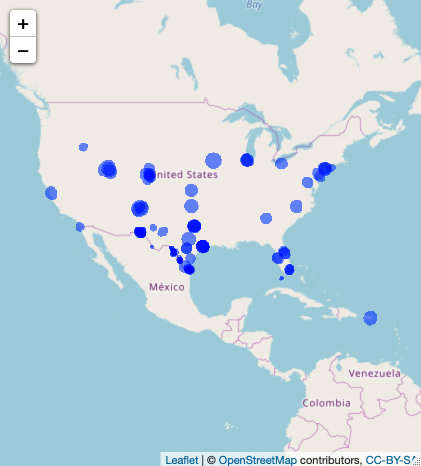
\includegraphics[width=8cm]{../analysis/Output/img/SpanishContours.png}
\end{figure} 

In the case of Spanish language TV in particular, this should allow me to examine its causal effect on Hispanic populations for spatially located outcomes, such as public schooling results. It's worth noting that these contours are purely determined by an algorithm that looks at things like local elevation and antennae strength, so that the cutoffs are located in more or less random locations, and that coverage is large enough that these contours tend to cut across towns and suburbs, rather than cities. % Finally, regressions using US census data indicate that Hispanic people do not migrate across counties in response to these contours.

A standard regression thus looks like restricting the universe of schools to only those within a small radius of the contour boundary, where the key independent variable of interest is an indicator for the school being inside or outside the boundary, interacted with the distance to the boundary:
\[ Y_i^{j,k} = \beta_0 + \beta \mathbb{I}[InsideContour_i] \times Distance_i + \gamma X_i + \delta Z^j + \epsilon_i^k \, \, \, \, \, \, \, \epsilon \stackrel{iid}{\sim}   N(0,\sigma_i^{k^2})\]

where $Y_i$ is an outcome for school $i$ in county $j$ and school district $k$, $X$ is a vector of school-level controls, and $Z$ is a vector of county-level controls. Errors are often clustered by school district, meaning that $Corr(\sigma_i^k, \sigma_{i'}^k) \neq 0$ is permissible.

When the outcome variable is a binary variable, the model instead follows:
\[\mathbb{P}(Y_i^j = 1 | X,Z) = \frac{\exp[\beta_0 + \beta \mathbb{I}[InsideContour_i] \times Distance_i + \gamma X_i + \delta Z^j ] }{ 1 + \exp[\beta_0 + \beta \mathbb{I}[InsideContour_i] \times Distance_i + \gamma X_i + \delta Z^j ]}\]

for a logistic/logit regression. 

\subsection*{Data}

Data for the instrument comes from both the FCC and TMS (a telecommunications company that was kind enough to let me use their API for free). The relevant data here is essentially just the coverage contour spatial data and the broadcast language of the station.


The data on public schools comes from the US government's CRDC (Civil Rights Data Collection) dataset. It's a very large dataset with over 500 outcome/control variables (the vast majority of these are not suitable as controls for one another in this setting), and importantly, it breaks down all major variables of interest by ethnicity. These are all at the school level, and the geographic location of these schools is mapped using ArcGIS. 

\begin{figure}[!hbtp]
\centering
\caption{Map of School Districts in the US}
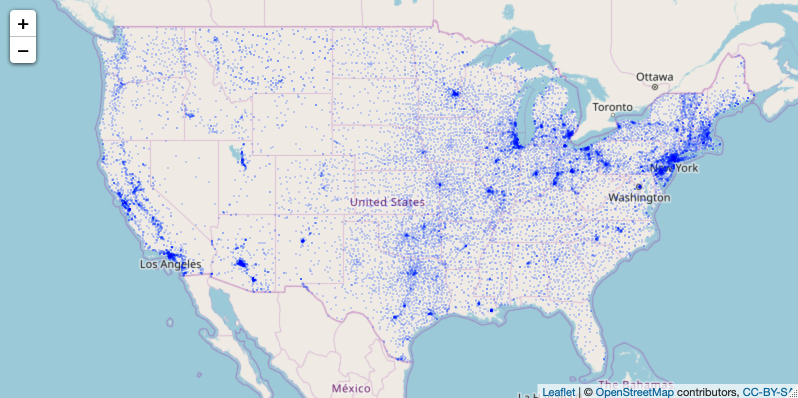
\includegraphics[width=12cm]{../analysis/Output/img/LEAMap.png}
\end{figure} 

To limit the problem of multiple testing, I limit analysis to two outcomes of interest: chronic absenteeism and out-of-school suspensions. Both are important outcomes in and of themselves, and one can reasonably interpret them for being good proxies for level of engagement in school (absenteeism) and disciplinary/behavioral issues (suspensions).

Several variables that frequently appear as controls include the number of teachers, students, Hispanic students, and whether the school services grades 1/6/9. The number of teachers and students give us (roughly) a school's size and how well staffed it is, which maybe a confound, given that it probably affects the outcomes (larger schools or ones with fewer teachers might have more trouble enforcing discipline), and is related to distance from the contour boundary (more rural/urban schools are different in size). A similar story can be told with Hispanic students and whether the school contains a primary/middle/high school.

Additional controls like population, income, density of Hispanic population etc. at the county level are from IPUMS. These variables are also added as controls, given their ability to affect both outcome and distance/presence of television (for instance, higher incomes might be associated with better upbringing or threat of lawsuit, decreasing school suspensions, while they might also be associated with the suburbs/owning more televisions to watch shows etc.) 

By limiting the analysis to a small distance from the contour boundary ($100$ KM/63 miles by default), we also minimize the potential concerns of omitted variable bias etc., as these schools must now be at least fairly close to one another, meaning that they probably share many overarching characteristics.

Some summary statistics of interest are presented below:


% Table created by stargazer v.5.2.2 by Marek Hlavac, Harvard University. E-mail: hlavac at fas.harvard.edu
% Date and time: Fri, Dec 13, 2019 - 20:45:59
\begin{table}[!htbp] \centering 
  \caption{School-District Level Summary Statistics} 
  \label{} 
\begin{tabular}{@{\extracolsep{5pt}}lccccccc} 
\\[-1.8ex]\hline 
\hline \\[-1.8ex] 
Statistic & \multicolumn{1}{c}{N} & \multicolumn{1}{c}{Mean} & \multicolumn{1}{c}{St. Dev.} & \multicolumn{1}{c}{Min} & \multicolumn{1}{c}{Pctl(25)} & \multicolumn{1}{c}{Pctl(75)} & \multicolumn{1}{c}{Max} \\ 
\hline \\[-1.8ex] 
Distance to Boundary & 17,280 & 136.855 & 146.751 & 0.000 & 15.786 & 217.567 & 806.543 \\ 
SLTV Coverage Dummy & 17,280 & 0.292 & 0.455 & 0.000 & 0.000 & 1.000 & 1.000 \\ 
\% County Hispanic & 17,280 & 7.051 & 11.950 & 0.000 & 0.668 & 6.974 & 97.216 \\ 
Log(Population) & 17,280 & 11.618 & 1.840 & 5.869 & 10.242 & 13.110 & 15.997 \\ 
Log(Income) & 17,280 & 9.428 & 0.257 & 7.976 & 9.257 & 9.593 & 10.245 \\ 
\hline \\[-1.8ex] 
\multicolumn{8}{l}{\textit{Note:} Distance to SLTV Boundary measured in KM} \\ 
\end{tabular} 
\end{table} 


% Table created by stargazer v.5.2.2 by Marek Hlavac, Harvard University. E-mail: hlavac at fas.harvard.edu
% Date and time: Fri, Dec 13, 2019 - 22:32:28
\begin{table}[!htbp] \centering 
  \caption{School Level Summary Statistics} 
  \label{} 
\begin{tabular}{@{\extracolsep{5pt}}lccccccc} 
\\[-1.8ex]\hline 
\hline \\[-1.8ex] 
Statistic & \multicolumn{1}{c}{N} & \multicolumn{1}{c}{Mean} & \multicolumn{1}{c}{St. Dev.} & \multicolumn{1}{c}{Min} & \multicolumn{1}{c}{Pctl(25)} & \multicolumn{1}{c}{Pctl(75)} & \multicolumn{1}{c}{Max} \\ 
\hline \\[-1.8ex] 
Total Students & 96,349 & 524.859 & 449.354 & 2.000 & 254.000 & 662.000 & 14,164.000 \\ 
\# Hispanic Students & 91,019 & 143.195 & 243.873 & 2.000 & 13.000 & 166.000 & 7,675.000 \\ 
Contains Grade 1 & 96,350 & 0.538 & 0.499 & 0 & 0 & 1 & 1 \\ 
Contains Grade 6 & 96,350 & 0.364 & 0.481 & 0 & 0 & 1 & 1 \\ 
Contains Grade 9 & 96,350 & 0.253 & 0.435 & 0 & 0 & 1 & 1 \\ 
Hispanic Suspension Dummy & 94,535 & 0.382 & 0.486 & 0.000 & 0.000 & 1.000 & 1.000 \\ 
Hispanic Chronic Absentees & 94,540 & 22.920 & 57.838 & 0.000 & 0.000 & 22.000 & 2,131.000 \\ 
\# Teachers & 93,934 & 35.219 & 33.892 & 1.000 & 19.000 & 44.000 & 6,031.000 \\ 
\hline \\[-1.8ex] 
\multicolumn{8}{l}{\textit{Note:} Dummies indicate whether event occurred in the school over the past year} \\ 
\end{tabular} 
\end{table} 

\clearpage

\section*{Absentees}

In the following regressions, I examine the number of Hispanic students identified as chronically absent (missing more than 15 days of school in a year). Running a regression on an untransformed variable leads to problems easily solved by a log transform (right skew, heteroskedasticity with variance increasing in the predicted outcome). However, there are a fair number of 0s, so instead of a log, the comparable Inverse Hyperbolic Sine (IHS) transform is used instead:


% Table created by stargazer v.5.2.2 by Marek Hlavac, Harvard University. E-mail: hlavac at fas.harvard.edu
% Date and time: Fri, Dec 13, 2019 - 22:51:54
\begin{table}[!htbp] \centering 
  \caption{Effect of TV on Hispanic Absentees} 
  \label{} 
\begin{tabular}{@{\extracolsep{-2pt}}lccccc} 
\\[-1.8ex]\hline 
\hline \\[-1.8ex] 
 & \multicolumn{5}{c}{\textit{Dependent variable:}} \\ 
\cline{2-6} 
\\[-1.8ex] & \multicolumn{5}{c}{IHS(Hispanic Absentees)} \\ 
\\[-1.8ex] & (1) & (2) & (3) & (4) & (5)\\ 
\hline \\[-1.8ex] 
 TV Dummy & 1.062$^{***}$ & 0.399$^{***}$ & 0.254$^{***}$ & 0.120$^{***}$ & 0.065$^{***}$ \\ 
  & (0.022) & (0.023) & (0.023) & (0.021) & (0.020) \\ 
  & & & & & \\ 
 TV Dummy $\times$ Distance to Boundary & $-$0.002$^{***}$ & 0.003$^{***}$ & 0.004$^{***}$ & 0.003$^{***}$ & 0.003$^{***}$ \\ 
  & (0.001) & (0.001) & (0.001) & (0.001) & (0.001) \\ 
  & & & & & \\ 
 Distance to Boundary (meters) & $-$0.007$^{***}$ & $-$0.006$^{***}$ & $-$0.006$^{***}$ & $-$0.005$^{***}$ & $-$0.005$^{***}$ \\ 
  & (0.0003) & (0.0003) & (0.0003) & (0.0003) & (0.0003) \\ 
  & & & & & \\ 
 Log(Population) &  & 0.209$^{***}$ & 0.125$^{***}$ & 0.107$^{***}$ & 0.049$^{***}$ \\ 
  &  & (0.005) & (0.006) & (0.006) & (0.005) \\ 
  & & & & & \\ 
 \% County Hispanic &  & 2.849$^{***}$ & 3.655$^{***}$ & 3.530$^{***}$ & 1.761$^{***}$ \\ 
  &  & (0.051) & (0.060) & (0.054) & (0.055) \\ 
  & & & & & \\ 
 Log(Income) &  &  & 0.859$^{***}$ & 0.551$^{***}$ & 0.837$^{***}$ \\ 
  &  &  & (0.035) & (0.032) & (0.029) \\ 
  & & & & & \\ 
 \# Teachers at School &  &  &  & 0.023$^{***}$ & 0.005$^{***}$ \\ 
  &  &  &  & (0.0002) & (0.0004) \\ 
  & & & & & \\ 
 \# Hispanic Students &  &  &  &  & 0.003$^{***}$ \\ 
  &  &  &  &  & (0.00004) \\ 
  & & & & & \\ 
 Total Students &  &  &  &  & 0.0004$^{***}$ \\ 
  &  &  &  &  & (0.00003) \\ 
  & & & & & \\ 
 Contains Grade 6 &  &  &  &  & $-$0.073$^{***}$ \\ 
  &  &  &  &  & (0.013) \\ 
  & & & & & \\ 
\hline \\[-1.8ex] 
Observations & 45,952 & 45,952 & 45,952 & 45,952 & 45,952 \\ 
R$^{2}$ & 0.122 & 0.212 & 0.222 & 0.368 & 0.466 \\ 
Adjusted R$^{2}$ & 0.122 & 0.212 & 0.222 & 0.368 & 0.466 \\ 
\hline 
\hline \\[-1.8ex] 
\textit{Note:}  & \multicolumn{5}{r}{$^{*}$p$<$0.1; $^{**}$p$<$0.05; $^{***}$p$<$0.01} \\ 
\end{tabular} 
\end{table} 

\clearpage
%% MULTIPLE DISTANCES
Column 1 presents the most simple model without any additional controls. The figure below presents some regression diagnostics (the fitted outcome against studentized residuals, a histogram of the studentized residuals, and a QQ plot of the studentized residuals): 

\begin{figure}[!hbtp]
\centering
\caption{Table 3, Column 1 Regression Diagnostics}
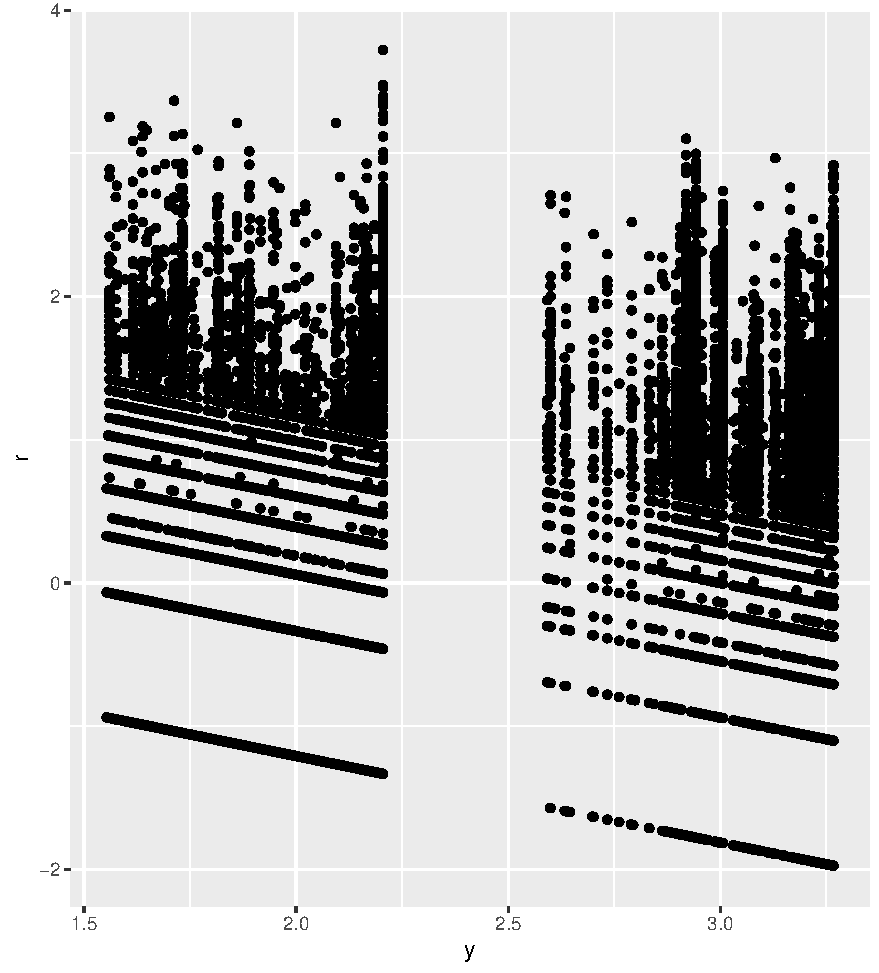
\includegraphics[width=5.5cm]{../explore/Output/diagnostics/edu_AbsOLS1Plot.pdf}
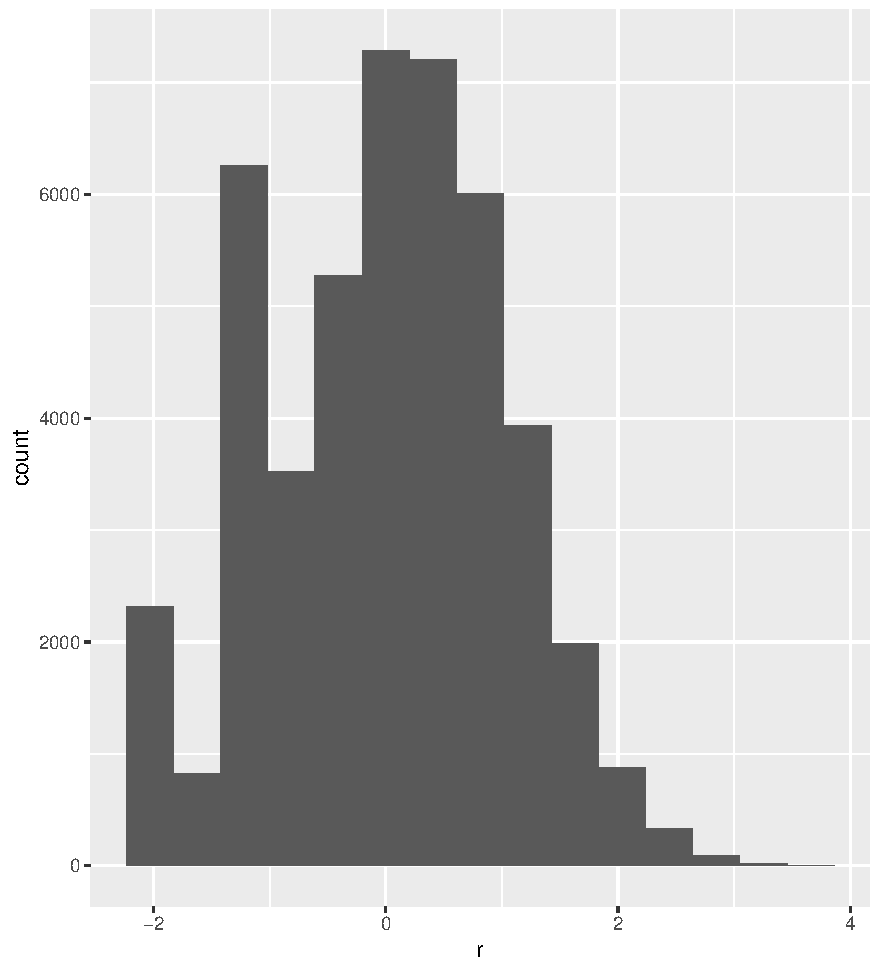
\includegraphics[width=5.5cm]{../explore/Output/diagnostics/edu_AbsOLS1Hist.pdf}
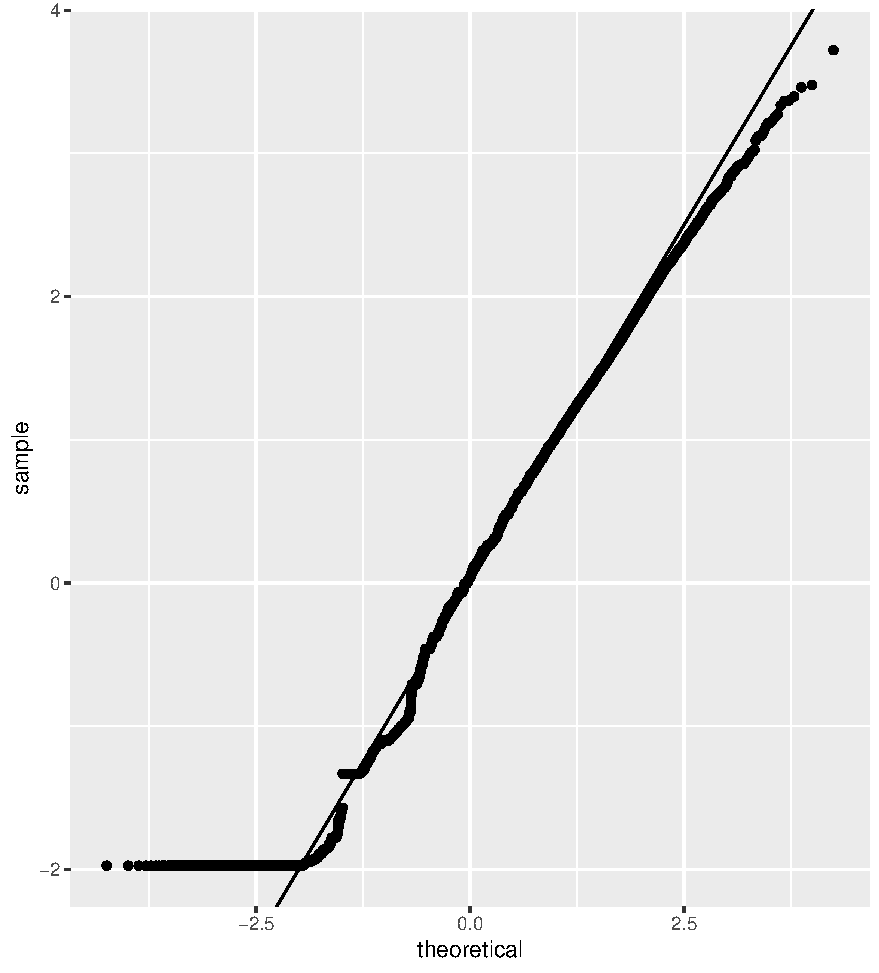
\includegraphics[width=5.5cm]{../explore/Output/diagnostics/edu_AbsOLS1QQ.pdf}
\end{figure} 

The histogram and QQ plots look roughly normal, but the presence of a large number of 0s creates a skew in the data that can be difficult to correct for. Nonetheless, adding extra controls helps to address this problem, as shown with the column 3 data:

\begin{figure}[!hbtp]
\centering
\caption{Table 3, Column 3 Regression Diagnostics}
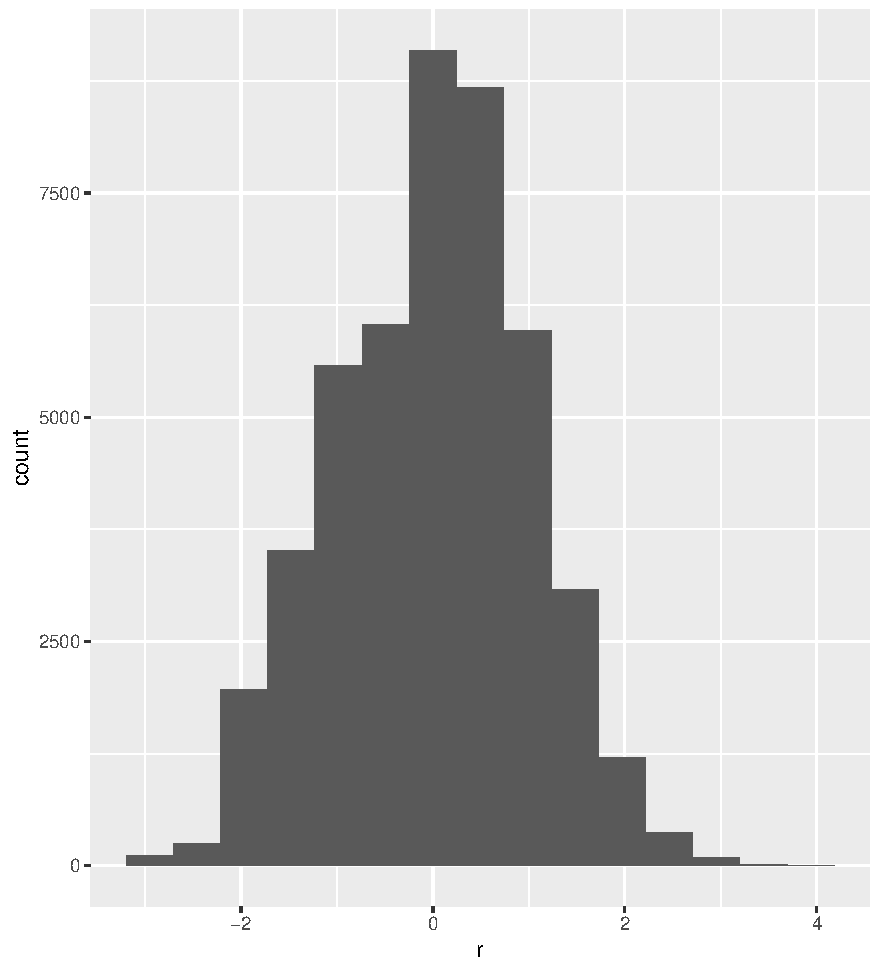
\includegraphics[width=4cm]{../explore/Output/diagnostics/edu_AbsOLS3Hist.pdf}
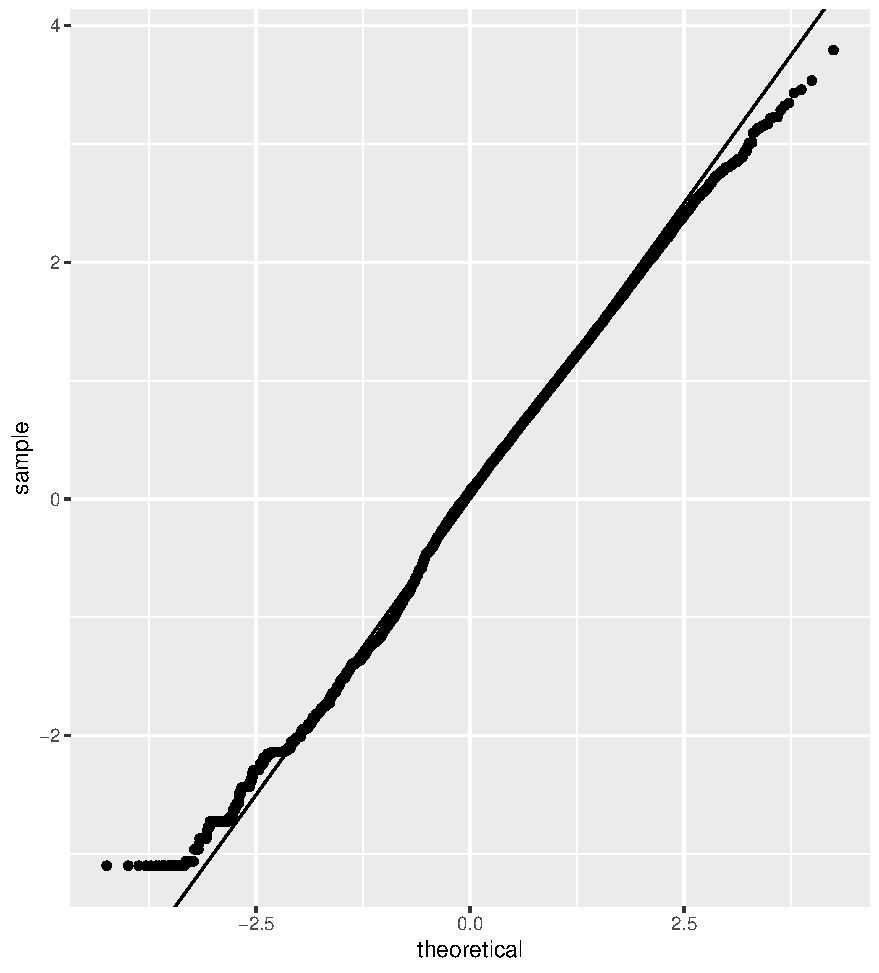
\includegraphics[width=4cm]{../explore/Output/diagnostics/edu_AbsOLS3QQ.pdf}
\end{figure}


Column (5) adds in a number of school-level controls. However, the universe of these is large, and they are potentially collinear. Thus, the variables present in the regression are selected using forward stepwise BIC. Further, employing a partial F-test also justifies each successive addition of variables across the columns of this regression.

To check for robustness, these results are replicated using different specifications. Column 1 is identical to Table 3, Column 5, with the distance cutoff for inclusion in the regression discontinuity set at 100 KM. This is reduced to 75 KM in column 2 and 50 in column 3. Column 4 clusters errors by ZIP code instead. While the directional results hold, significance is lost due to the lower amount of information linked with having fewer observations, or fewer clusters.

% Table created by stargazer v.5.2.2 by Marek Hlavac, Harvard University. E-mail: hlavac at fas.harvard.edu
% Date and time: Fri, Dec 13, 2019 - 23:19:47
\begin{table}[!htbp] \centering 
  \caption{Effect of TV on Hispanic Absentees} 
  \label{} 
\begin{tabular}{@{\extracolsep{-2pt}}lcccc} 
\\[-1.8ex]\hline 
\hline \\[-1.8ex] 
 & \multicolumn{4}{c}{\textit{Dependent variable:}} \\ 
\cline{2-5} 
\\[-1.8ex] & \multicolumn{4}{c}{IHS(Hispanic Absentees)} \\ 
\\[-1.8ex] & (1) & (2) & (3) & (4)\\ 
\hline \\[-1.8ex] 
 TV Dummy & 0.065$^{***}$ & 0.060$^{***}$ & 0.017 & 0.055 \\ 
  & (0.020) & (0.020) & (0.021) & (0.073) \\ 
  & & & & \\ 
 TV Dummy $\times$ Distance to Boundary & 0.003$^{***}$ & 0.004$^{***}$ & 0.006$^{***}$ & 0.003 \\ 
  & (0.001) & (0.001) & (0.001) & (0.002) \\ 
  & & & & \\ 
 Distance to Boundary (meters) & $-$0.005$^{***}$ & $-$0.007$^{***}$ & $-$0.008$^{***}$ & $-$0.005$^{***}$ \\ 
  & (0.0003) & (0.0004) & (0.001) & (0.001) \\ 
  & & & & \\ 
 Log(Population) & 0.049$^{***}$ & 0.046$^{***}$ & 0.064$^{***}$ & 0.050$^{**}$ \\ 
  & (0.005) & (0.006) & (0.006) & (0.023) \\ 
  & & & & \\ 
 \% County Hispanic & 1.761$^{***}$ & 1.761$^{***}$ & 1.824$^{***}$ & 1.757$^{***}$ \\ 
  & (0.055) & (0.056) & (0.058) & (0.428) \\ 
  & & & & \\ 
 Log(Income) & 0.837$^{***}$ & 0.833$^{***}$ & 0.855$^{***}$ & 0.846$^{**}$ \\ 
  & (0.029) & (0.030) & (0.032) & (0.331) \\ 
  & & & & \\ 
 \# Teachers at School & 0.005$^{***}$ & 0.005$^{***}$ & 0.004$^{***}$ & 0.005$^{***}$ \\ 
  & (0.0004) & (0.0005) & (0.0005) & (0.001) \\ 
  & & & & \\ 
 \# Hispanic Students & 0.003$^{***}$ & 0.003$^{***}$ & 0.003$^{***}$ & 0.003$^{***}$ \\ 
  & (0.00004) & (0.00004) & (0.00004) & (0.0002) \\ 
  & & & & \\ 
 Total Students & 0.0004$^{***}$ & 0.0004$^{***}$ & 0.0005$^{***}$ & 0.0004$^{***}$ \\ 
  & (0.00003) & (0.00003) & (0.00003) & (0.0001) \\ 
  & & & & \\ 
 Contains Grade 6 & $-$0.073$^{***}$ & $-$0.079$^{***}$ & $-$0.084$^{***}$ & $-$0.079$^{***}$ \\ 
  & (0.013) & (0.013) & (0.015) & (0.024) \\ 
  & & & & \\ 
\hline \\[-1.8ex] 
Observations & 45,952 & 41,249 & 35,276 & 45,784 \\ 
R$^{2}$ & 0.466 & 0.465 & 0.458 & 0.468 \\ 
Adjusted R$^{2}$ & 0.466 & 0.465 & 0.458 & 0.467 \\ 
\hline 
\hline \\[-1.8ex] 
\textit{Note:}  & \multicolumn{4}{r}{$^{*}$p$<$0.1; $^{**}$p$<$0.05; $^{***}$p$<$0.01} \\ 
\end{tabular} 
\end{table} 

%
% Table created by stargazer v.5.2.2 by Marek Hlavac, Harvard University. E-mail: hlavac at fas.harvard.edu
% Date and time: Fri, Dec 13, 2019 - 23:18:07
\begin{table}[!htbp] \centering 
  \caption{Effect of TV on Hispanic \% Harassment Victims} 
  \label{} 
\begin{tabular}{@{\extracolsep{-2pt}}lccccc} 
\\[-1.8ex]\hline 
\hline \\[-1.8ex] 
 & \multicolumn{5}{c}{\textit{Dependent variable:}} \\ 
\cline{2-6} 
\\[-1.8ex] & \multicolumn{5}{c}{ihs\_absent\_hi} \\ 
\\[-1.8ex] & (1) & (2) & (3) & (4) & (5)\\ 
\hline \\[-1.8ex] 
 TV Dummy & 1.062$^{***}$ & 0.398$^{***}$ & 0.251$^{***}$ & 0.111 & 0.055 \\ 
  & (0.167) & (0.096) & (0.089) & (0.087) & (0.073) \\ 
  & & & & & \\ 
 TV Dummy $\times$ Distance to Boundary & $-$0.002 & 0.003 & 0.004 & 0.003 & 0.003 \\ 
  & (0.004) & (0.003) & (0.003) & (0.003) & (0.002) \\ 
  & & & & & \\ 
 Distance to Boundary (meters) & $-$0.007$^{***}$ & $-$0.006$^{***}$ & $-$0.006$^{***}$ & $-$0.005$^{***}$ & $-$0.005$^{***}$ \\ 
  & (0.001) & (0.001) & (0.001) & (0.001) & (0.001) \\ 
  & & & & & \\ 
 Log(Population) &  & 0.209$^{***}$ & 0.126$^{***}$ & 0.108$^{***}$ & 0.050$^{**}$ \\ 
  &  & (0.024) & (0.023) & (0.025) & (0.023) \\ 
  & & & & & \\ 
 \% County Hispanic &  & 2.848$^{***}$ & 3.655$^{***}$ & 3.530$^{***}$ & 1.757$^{***}$ \\ 
  &  & (0.197) & (0.305) & (0.409) & (0.428) \\ 
  & & & & & \\ 
 Log(Income) &  &  & 0.862$^{***}$ & 0.558$^{*}$ & 0.846$^{**}$ \\ 
  &  &  & (0.226) & (0.317) & (0.331) \\ 
  & & & & & \\ 
 \# Teachers at School &  &  &  & 0.023$^{***}$ & 0.005$^{***}$ \\ 
  &  &  &  & (0.001) & (0.001) \\ 
  & & & & & \\ 
 hisp\_students &  &  &  &  & 0.003$^{***}$ \\ 
  &  &  &  &  & (0.0002) \\ 
  & & & & & \\ 
 total\_students &  &  &  &  & 0.0004$^{***}$ \\ 
  &  &  &  &  & (0.0001) \\ 
  & & & & & \\ 
 SCH\_GRADE\_G06Yes &  &  &  &  & $-$0.079$^{***}$ \\ 
  &  &  &  &  & (0.024) \\ 
  & & & & & \\ 
\hline \\[-1.8ex] 
Observations & 45,784 & 45,784 & 45,784 & 45,784 & 45,784 \\ 
R$^{2}$ & 0.122 & 0.213 & 0.223 & 0.369 & 0.468 \\ 
Adjusted R$^{2}$ & 0.122 & 0.213 & 0.223 & 0.368 & 0.467 \\ 
\hline 
\hline \\[-1.8ex] 
\textit{Note:}  & \multicolumn{5}{r}{$^{*}$p$<$0.1; $^{**}$p$<$0.05; $^{***}$p$<$0.01} \\ 
\end{tabular} 
\end{table} 


\begin{figure}[!hbtp]
\centering
\caption{Table 3, Column 5 Regression Diagnostics}
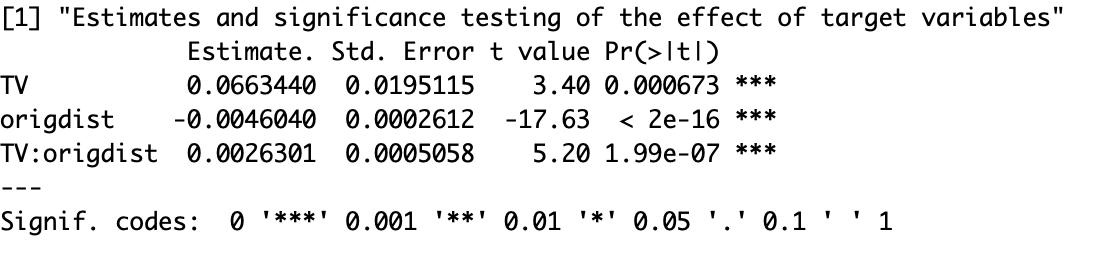
\includegraphics[width=12cm]{../explore/Output/regs/edu_absLasso}
\end{figure} 

Finally, a regression utilizing LASSO is presented; the information matches what we saw in the prior regressions, with the effect of television and the interaction both being positive and significant for $\alpha = .1$.

Given the relative consistency of these results, how should we interpret them? If you buy that the regression discontinuity operates, whether in a hard cut-off sense associated with the FCC regulation, or in the weaker, decaying signal over distance sense, then this implies that the presence of Spanish Language Television causes more Hispanic students to become chronically absent.

This is immediately clear from the sign on the coefficient of TV, and note that the interaction is positive, meaning that for those within the contour, being further away from the boundary (i.e. closer to the source signal) causes higher absenteeism; this sign on distance flips for those outside the TV contour.

The magnitude of this effect is fair. Given the comparability of IHS and log, the point estimates ranging from around $.05$ to $.25$ represents a similar percentage increase in chronic absenteeism due to the presence of SLTV, which one could reasonably think would be large enough to be worth worrying about. 



\clearpage

\subsection*{Suspensions}

In the following regressions, I examine out of school suspensions (these do not contribute towards absenteeism). First, with a logit approach using a dummy for a school in the past year ever having a Hispanic student receiving at least one out of school suspension: 


% Table created by stargazer v.5.2.2 by Marek Hlavac, Harvard University. E-mail: hlavac at fas.harvard.edu
% Date and time: Fri, Dec 13, 2019 - 19:09:45
\begin{table}[!htbp] \centering 
  \caption{Effect of TV on Hispanic Out of School Suspension Dummy} 
  \label{} 
\begin{tabular}{@{\extracolsep{-2pt}}lccccc} 
\\[-1.8ex]\hline 
\hline \\[-1.8ex] 
 & \multicolumn{5}{c}{\textit{Dependent variable:}} \\ 
\cline{2-6} 
\\[-1.8ex] & \multicolumn{5}{c}{hisp\_OOSDum} \\ 
\\[-1.8ex] & (1) & (2) & (3) & (4) & (5)\\ 
\hline \\[-1.8ex] 
 TV Dummy & 0.397$^{***}$ & 0.092$^{***}$ & 0.204$^{***}$ & 0.064$^{*}$ & $-$0.006 \\ 
  & (0.027) & (0.030) & (0.031) & (0.033) & (0.035) \\ 
  & & & & & \\ 
 TV Dummy $\times$ Distance to Boundary & 0.003$^{***}$ & 0.006$^{***}$ & 0.005$^{***}$ & 0.004$^{***}$ & 0.005$^{***}$ \\ 
  & (0.001) & (0.001) & (0.001) & (0.001) & (0.001) \\ 
  & & & & & \\ 
 Distance to Boundary (meters) & $-$0.005$^{***}$ & $-$0.004$^{***}$ & $-$0.004$^{***}$ & $-$0.004$^{***}$ & $-$0.003$^{***}$ \\ 
  & (0.0004) & (0.0004) & (0.0004) & (0.0005) & (0.0005) \\ 
  & & & & & \\ 
 Log(Population) &  & 0.074$^{***}$ & 0.138$^{***}$ & 0.135$^{***}$ & 0.102$^{***}$ \\ 
  &  & (0.007) & (0.008) & (0.009) & (0.010) \\ 
  & & & & & \\ 
 \% County Hispanic &  & 1.714$^{***}$ & 1.127$^{***}$ & 1.210$^{***}$ & $-$1.383$^{***}$ \\ 
  &  & (0.069) & (0.081) & (0.088) & (0.109) \\ 
  & & & & & \\ 
 Log(Income) &  &  & $-$0.664$^{***}$ & $-$1.180$^{***}$ & $-$1.024$^{***}$ \\ 
  &  &  & (0.046) & (0.050) & (0.054) \\ 
  & & & & & \\ 
 \# Teachers at School &  &  &  & 0.031$^{***}$ & 0.010$^{***}$ \\ 
  &  &  &  & (0.0005) & (0.001) \\ 
  & & & & & \\ 
 \# Hispanic Students &  &  &  &  & 0.005$^{***}$ \\ 
  &  &  &  &  & (0.0001) \\ 
  & & & & & \\ 
 Total Students &  &  &  &  & 0.0004$^{***}$ \\ 
  &  &  &  &  & (0.0001) \\ 
  & & & & & \\ 
 \# Students in Grade 1 &  &  &  &  & $-$0.887$^{***}$ \\ 
  &  &  &  &  & (0.027) \\ 
  & & & & & \\ 
 \# Students in Grade 6 &  &  &  &  & 0.299$^{***}$ \\ 
  &  &  &  &  & (0.024) \\ 
  & & & & & \\ 
 \# Students in Grade 9 &  &  &  &  & 0.126$^{***}$ \\ 
  &  &  &  &  & (0.031) \\ 
  & & & & & \\ 
\hline \\[-1.8ex] 
Observations & 45,947 & 45,947 & 45,947 & 45,947 & 45,947 \\ 
Log Likelihood & $-$30,733.950 & $-$30,315.250 & $-$30,211.380 & $-$27,500.700 & $-$24,898.820 \\ 
Akaike Inf. Crit. & 61,475.890 & 60,642.500 & 60,436.760 & 55,017.410 & 49,823.650 \\ 
\hline 
\hline \\[-1.8ex] 
\textit{Note:}  & \multicolumn{5}{r}{$^{*}$p$<$0.1; $^{**}$p$<$0.05; $^{***}$p$<$0.01} \\ 
\end{tabular} 
\end{table} 

\clearpage

Column 1 presents the most simple model without any additional controls. The figure below presents some regression diagnostics (the fitted outcome against studentized residuals, a histogram of the studentized residuals, and a QQ plot of the studentized residuals): 

\begin{figure}[!hbtp]
\centering
\caption{Table 5, Column 1 Regression Diagnostics}
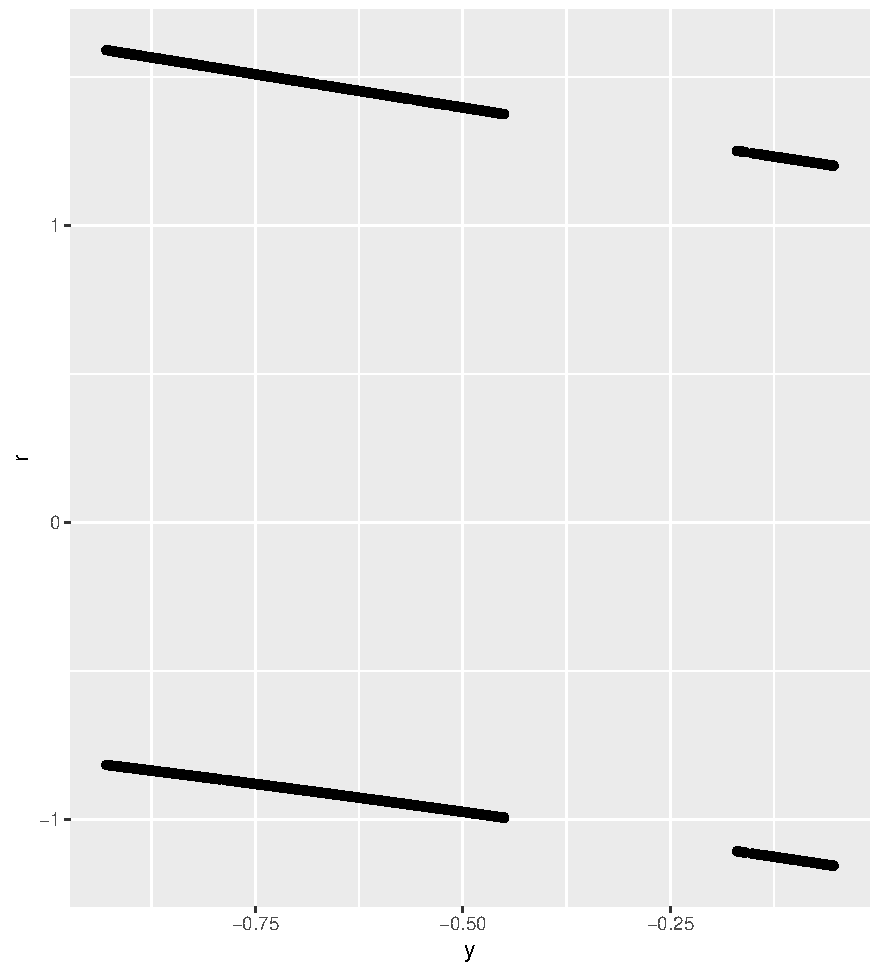
\includegraphics[width=6cm]{../explore/Output/diagnostics/edu_OOSLogit1Plot.pdf}
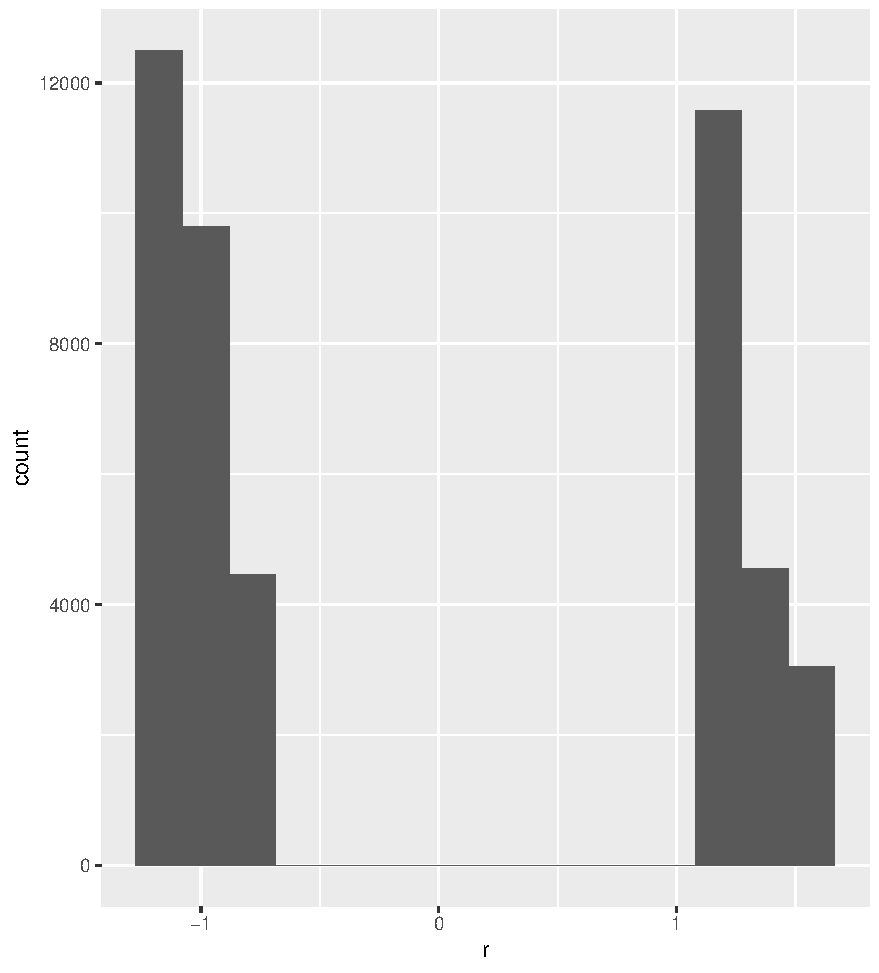
\includegraphics[width=6cm]{../explore/Output/diagnostics/edu_OOSLogit1Hist.pdf}
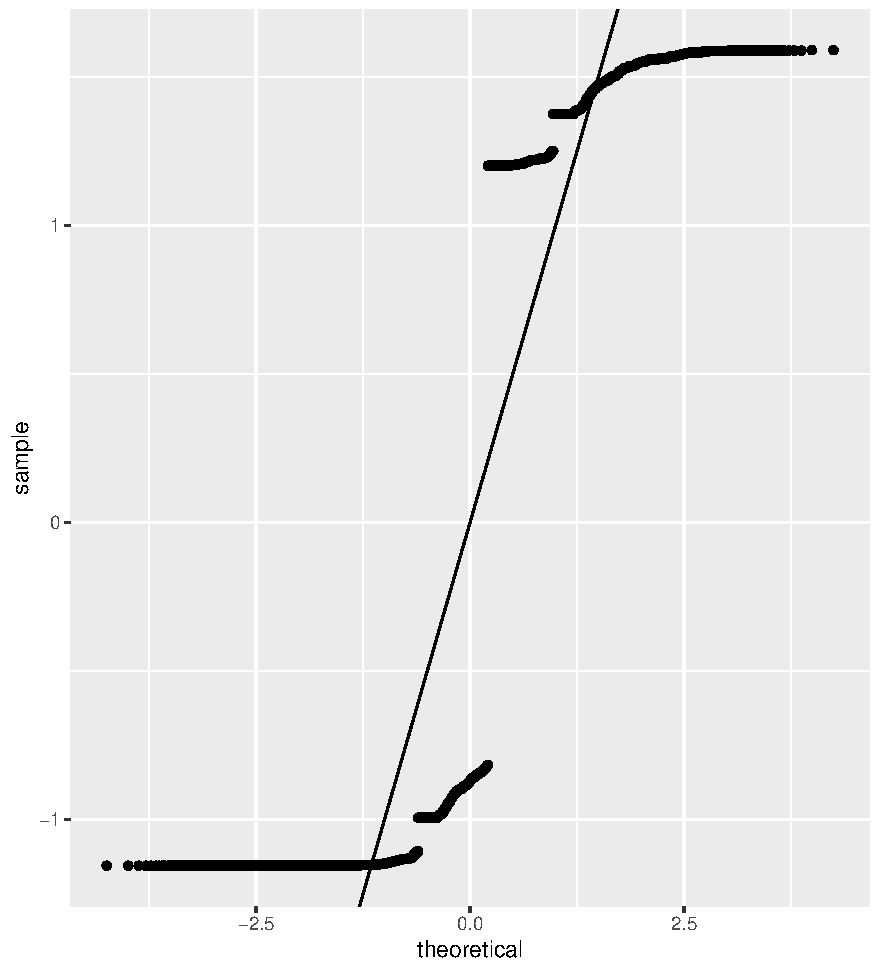
\includegraphics[width=6cm]{../explore/Output/diagnostics/edu_OOSLogit1QQ.pdf}
\end{figure} 
It is clear that are outstanding issues with the regression: they are clumped into two groups based on whether the outcome holds or not. This indicates that there are still large underlying sources of variation that are not being captured by the regression itself. Given the spatial nature of the identification method, it is natural to control for the demographic features of the areas in which the schools are located, which is what is done in columns (2) and (3). 

The key result, that television drives negative outcomes, is nonetheless present in this first regression: this is visible from the positive television dummy, but also from the interaction term. If there is indeed an effect from television, we would expect these to be significant in the same direction, as the dummy captures the FCC regulation imposed cutoff, while there is also a natural decay in signal strength over distance.  

Column (5) adds in school-level controls. However, the universe of these is large, and they are potentially collinear.  Thus, the variables present in the regression are selected using forward stepwise BIC. While the partial $F$ test is inappropriate for this context (logit), employing a likelihood ratio test also justifies each successive addition of variables across the columns of this regression.
\clearpage

\begin{figure}[!hbtp]
\centering
\caption{Table 5, Column 5 Regression Diagnostics}
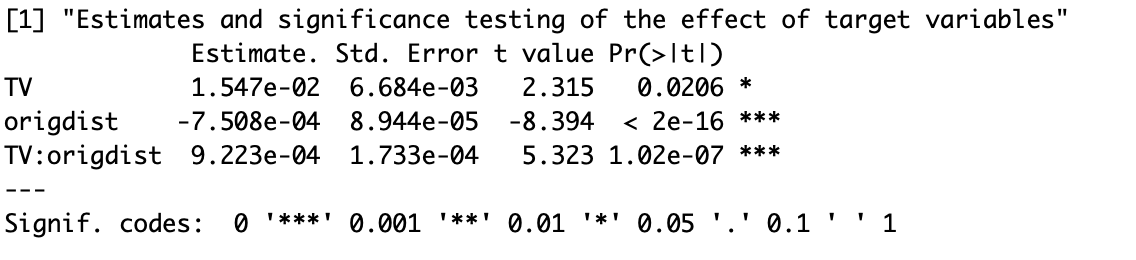
\includegraphics[width=12cm]{../explore/Output/regs/edu_OOSLasso}
\end{figure} 

Finally, a regression utilizing LASSO is presented; the information matches what we saw in the prior regressions, with the effect of television and the interaction both being positive and significant for $\alpha = .1$.

To verify that these additional controls have mitigated the concerns of non-normal residuals noted above, the diagnostics for the regression in column (5) are presented:

\begin{figure}[!hbtp]
\centering
\caption{Table 3, Column 5 Regression Diagnostics}
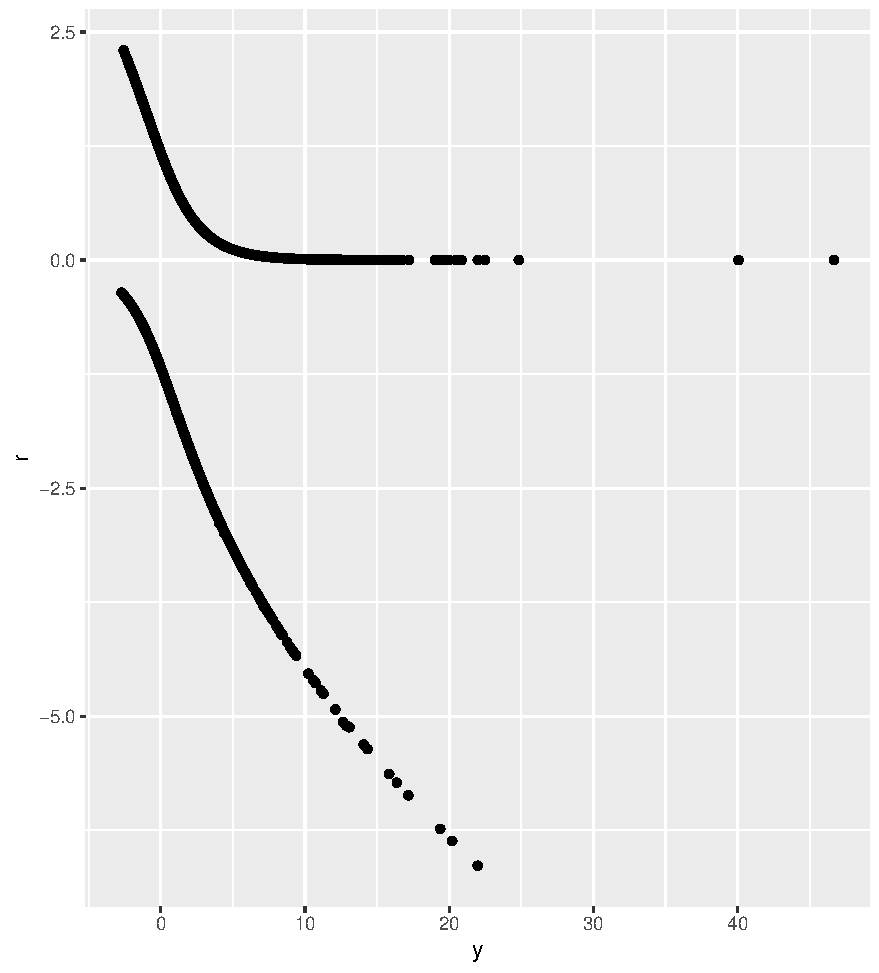
\includegraphics[width=6cm]{../explore/Output/diagnostics/edu_OOSLogit5Plot.pdf}
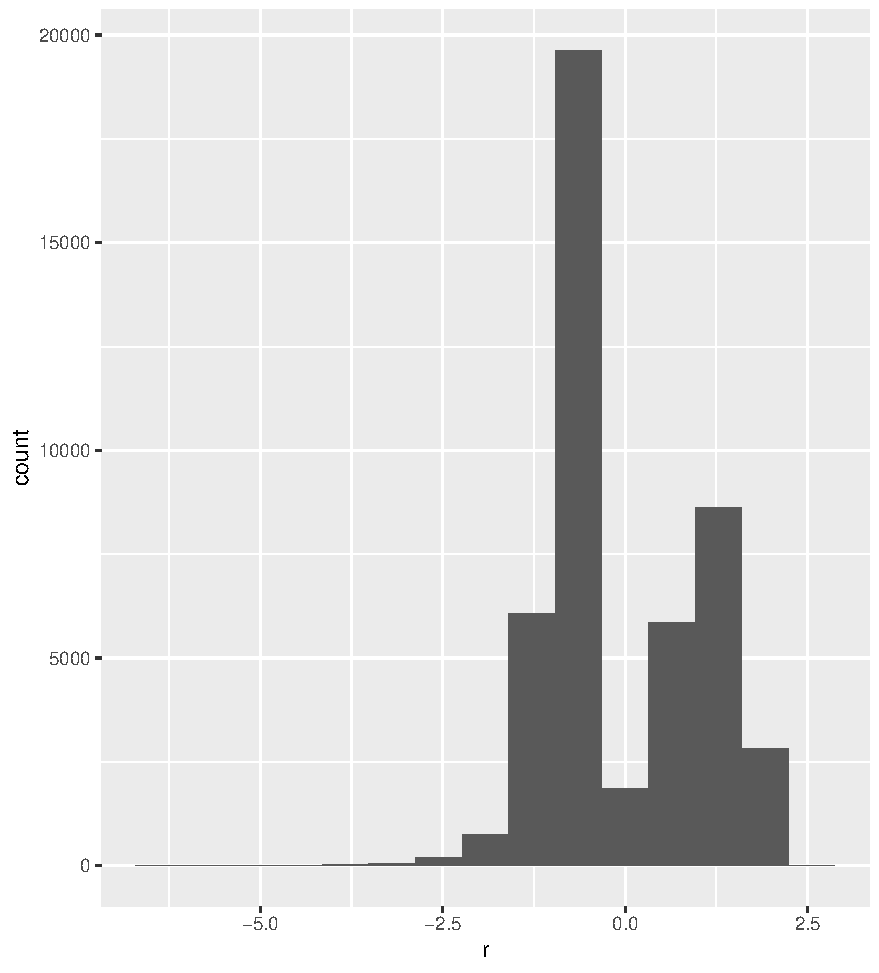
\includegraphics[width=6cm]{../explore/Output/diagnostics/edu_OOSLogit5Hist.pdf}
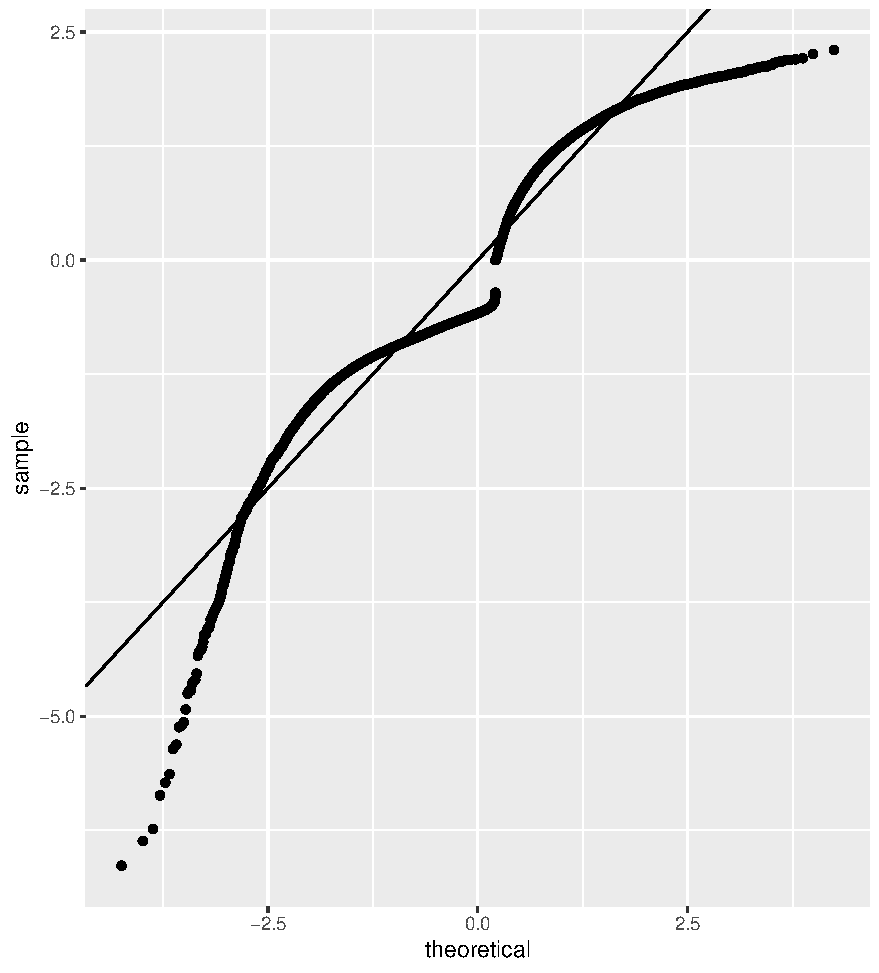
\includegraphics[width=6cm]{../explore/Output/diagnostics/edu_OOSLogit5QQ.pdf}
\end{figure} 

There are still two apparent clusters, but they are substantially less differentiated than in the simplest regression above. It's worth noting that most of the progress is made with the addition of county-level variables. Nonetheless, it still appears as if there is non-constant variance and an overall non-normal distribution. These problems can likely be attributed to the large number of 0s present in the regression (close to $2/3$ of values). Thus, a zero-inflated model with logit as the link and a Poisson distribution is used too, with results verified:


% Table created by stargazer v.5.2.2 by Marek Hlavac, Harvard University. E-mail: hlavac at fas.harvard.edu
% Date and time: Fri, Dec 13, 2019 - 22:26:07
\begin{table}[!htbp] \centering 
  \caption{Effect of TV on Hispanic Out of School Suspension Dummy, Zero-Inflated} 
  \label{} 
\begin{tabular}{@{\extracolsep{-2pt}}lccc} 
\\[-1.8ex]\hline 
\hline \\[-1.8ex] 
 & \multicolumn{3}{c}{\textit{Dependent variable:}} \\ 
\cline{2-4} 
\\[-1.8ex] & \multicolumn{3}{c}{\# Hispanic Out of School Suspensions} \\ 
\\[-1.8ex] & (1) & (2) & (3)\\ 
\hline \\[-1.8ex] 
 TV Dummy & 0.443$^{***}$ & 0.151$^{***}$ & 0.189$^{***}$ \\ 
  & (0.007) & (0.008) & (0.008) \\ 
  & & & \\ 
 TV Dummy $\times$ Distance to Boundary & 0.003$^{***}$ & 0.006$^{***}$ & 0.003$^{***}$ \\ 
  & (0.0002) & (0.0002) & (0.0002) \\ 
  & & & \\ 
 Distance to Boundary (meters) & $-$0.004$^{***}$ & $-$0.005$^{***}$ & $-$0.004$^{***}$ \\ 
  & (0.0001) & (0.0002) & (0.0002) \\ 
  & & & \\ 
 Log(Population) &  & 0.160$^{***}$ & 0.131$^{***}$ \\ 
  &  & (0.002) & (0.002) \\ 
  & & & \\ 
 \% County Hispanic &  & 0.735$^{***}$ & $-$0.215$^{***}$ \\ 
  &  & (0.018) & (0.018) \\ 
  & & & \\ 
 Log(Income) &  & $-$0.508$^{***}$ & $-$0.654$^{***}$ \\ 
  &  & (0.012) & (0.013) \\ 
  & & & \\ 
 \# Teachers at School &  &  & 0.004$^{***}$ \\ 
  &  &  & (0.00001) \\ 
  & & & \\ 
 \# Hispanic Students &  &  & 0.001 \\ 
  &  &  &  \\ 
  & & & \\ 
 Total Students &  &  & $-$0.0003 \\ 
  &  &  &  \\ 
  & & & \\ 
 Contains Grade 1 &  &  & $-$1.072$^{***}$ \\ 
  &  &  & (0.002) \\ 
  & & & \\ 
 Contains Grade 6 &  &  & 0.053$^{***}$ \\ 
  &  &  & (0.005) \\ 
  & & & \\ 
 Contains Grade 9 &  &  & 0.034$^{***}$ \\ 
  &  &  & (0.005) \\ 
  & & & \\ 
\hline \\[-1.8ex] 
Observations & 45,947 & 45,947 & 45,947 \\ 
Log Likelihood & $-$178,855.800 & $-$169,849.100 & $-$116,549.100 \\ 
\hline 
\hline \\[-1.8ex] 
\textit{Note:}  & \multicolumn{3}{r}{$^{*}$p$<$0.1; $^{**}$p$<$0.05; $^{***}$p$<$0.01} \\ 
\end{tabular} 
\end{table} 

\clearpage

From this, we glean that it is plausible for there to be a link between the presence of television and students acting out in ways leading to suspension. The conclusion is perhaps not as strong as in the case of absenteeism, given that the underlying regression assumptions are more frequently violated/in greater degree, but it is certainly suggestive of a similar story, where television causes greater rates of problematic behavior and hence suspension.

Though it cannot be confirmed that the driver of this mechanism is identity (this may simply be due to more television being watched), it does suggest that the media we broadcast and consume can have a potentially negative impact on educational attainment. I might take a look at some other related outcomes present in the dataset, and so would appreciate feedback apart from a letter grade! (Although I understand that this may not be possible given time constraints)

%
% Table created by stargazer v.5.2.2 by Marek Hlavac, Harvard University. E-mail: hlavac at fas.harvard.edu
% Date and time: Wed, Nov 13, 2019 - 15:16:32
\begin{table}[!htbp] \centering 
  \caption{GED Completions} 
  \label{} 
\begin{tabular}{@{\extracolsep{5pt}}lccccccc} 
\\[-1.8ex]\hline 
\hline \\[-1.8ex] 
Statistic & \multicolumn{1}{c}{N} & \multicolumn{1}{c}{Mean} & \multicolumn{1}{c}{St. Dev.} & \multicolumn{1}{c}{Min} & \multicolumn{1}{c}{Pctl(25)} & \multicolumn{1}{c}{Pctl(75)} & \multicolumn{1}{c}{Max} \\ 
\hline \\[-1.8ex] 
LEA\_GEDPART\_HI\_M & 656 & 12.901 & 77.293 & 0 & 0 & 5 & 1,550 \\ 
LEA\_GEDPART\_HI\_F & 656 & 10.869 & 66.649 & 0 & 0 & 5 & 1,136 \\ 
TOT\_GEDPART\_M & 656 & 53.639 & 173.840 & 2 & 10 & 51.2 & 3,485 \\ 
TOT\_GEDPART\_F & 656 & 39.765 & 136.175 & 0 & 5 & 37 & 2,225 \\ 
LEA\_GEDCRED\_HI\_M & 656 & 2.130 & 18.292 & $-$2 & $-$2 & $-$2 & 298 \\ 
LEA\_GEDCRED\_HI\_F & 656 & 1.201 & 16.312 & $-$2 & $-$2 & $-$2 & 253 \\ 
TOT\_GEDCRED\_M & 656 & 20.870 & 55.866 & 4 & 4 & 17 & 793 \\ 
TOT\_GEDCRED\_F & 656 & 13.791 & 43.218 & $-$2 & $-$2 & 11 & 619 \\ 
\hline \\[-1.8ex] 
\end{tabular} 
\end{table} 


%
% Table created by stargazer v.5.2.2 by Marek Hlavac, Harvard University. E-mail: hlavac at fas.harvard.edu
% Date and time: Wed, Nov 13, 2019 - 15:16:32
\begin{table}[!htbp] \centering 
  \caption{GED Completions} 
  \label{} 
\begin{tabular}{@{\extracolsep{5pt}}lccccccc} 
\\[-1.8ex]\hline 
\hline \\[-1.8ex] 
Statistic & \multicolumn{1}{c}{N} & \multicolumn{1}{c}{Mean} & \multicolumn{1}{c}{St. Dev.} & \multicolumn{1}{c}{Min} & \multicolumn{1}{c}{Pctl(25)} & \multicolumn{1}{c}{Pctl(75)} & \multicolumn{1}{c}{Max} \\ 
\hline \\[-1.8ex] 
LEA\_GEDPART\_HI\_M & 656 & 12.901 & 77.293 & 0 & 0 & 5 & 1,550 \\ 
LEA\_GEDPART\_HI\_F & 656 & 10.869 & 66.649 & 0 & 0 & 5 & 1,136 \\ 
TOT\_GEDPART\_M & 656 & 53.639 & 173.840 & 2 & 10 & 51.2 & 3,485 \\ 
TOT\_GEDPART\_F & 656 & 39.765 & 136.175 & 0 & 5 & 37 & 2,225 \\ 
LEA\_GEDCRED\_HI\_M & 656 & 2.130 & 18.292 & $-$2 & $-$2 & $-$2 & 298 \\ 
LEA\_GEDCRED\_HI\_F & 656 & 1.201 & 16.312 & $-$2 & $-$2 & $-$2 & 253 \\ 
TOT\_GEDCRED\_M & 656 & 20.870 & 55.866 & 4 & 4 & 17 & 793 \\ 
TOT\_GEDCRED\_F & 656 & 13.791 & 43.218 & $-$2 & $-$2 & 11 & 619 \\ 
\hline \\[-1.8ex] 
\end{tabular} 
\end{table} 






\end{document}
























